\documentclass{sigchi}

% Use this section to set the ACM copyright statement (e.g. for
% preprints).  Consult the conference website for the camera-ready
% copyright statement.

% Copyright
\CopyrightYear{2017}
%\setcopyright{acmcopyright}
\setcopyright{acmlicensed}
%\setcopyright{rightsretained}
%\setcopyright{usgov}
%\setcopyright{usgovmixed}
%\setcopyright{cagov}
%\setcopyright{cagovmixed}
% DOI
\doi{http://dx.doi.org/10.475/123_4}
% ISBN
\isbn{123-4567-24-567/08/06}
%Conference
\conferenceinfo{CHI'16,}{May 07--12, 2016, San Jose, CA, USA}
%Price
\acmPrice{\$15.00}

% Use this command to override the default ACM copyright statement
% (e.g. for preprints).  Consult the conference website for the
% camera-ready copyright statement.

%% HOW TO OVERRIDE THE DEFAULT COPYRIGHT STRIP --
%% Please note you need to make sure the copy for your specific
%% license is used here!
% \toappear{
% Permission to make digital or hard copies of all or part of this work
% for personal or classroom use is granted without fee provided that
% copies are not made or distributed for profit or commercial advantage
% and that copies bear this notice and the full citation on the first
% page. Copyrights for components of this work owned by others than ACM
% must be honored. Abstracting with credit is permitted. To copy
% otherwise, or republish, to post on servers or to redistribute to
% lists, requires prior specific permission and/or a fee. Request
% permissions from \href{mailto:Permissions@acm.org}{Permissions@acm.org}. \\
% \emph{CHI '16},  May 07--12, 2016, San Jose, CA, USA \\
% ACM xxx-x-xxxx-xxxx-x/xx/xx\ldots \$15.00 \\
% DOI: \url{http://dx.doi.org/xx.xxxx/xxxxxxx.xxxxxxx}
% }

% Arabic page numbers for submission.  Remove this line to eliminate
% page numbers for the camera ready copy
\pagenumbering{arabic}

% Load basic packages
\usepackage{balance}       % to better equalize the last page
\usepackage{graphics}      % for EPS, load graphicx instead 
\usepackage[T1]{fontenc}   % for umlauts and other diaeresis
\usepackage{txfonts}
\usepackage{mathptmx}
\usepackage[pdflang={en-US},pdftex]{hyperref}
\usepackage{color}
\usepackage{booktabs}
\usepackage{textcomp}

% Some optional stuff you might like/need.
\usepackage{microtype}        % Improved Tracking and Kerning
% \usepackage[all]{hypcap}    % Fixes bug in hyperref caption linking
\usepackage{ccicons}          % Cite your images correctly!
% \usepackage[utf8]{inputenc} % for a UTF8 editor only

% If you want to use todo notes, marginpars etc. during creation of
% your draft document, you have to enable the "chi_draft" option for
% the document class. To do this, change the very first line to:
% "\documentclass[chi_draft]{sigchi}". You can then place todo notes
% by using the "\todo{...}"  command. Make sure to disable the draft
% option again before submitting your final document.
\usepackage{todonotes}

% Paper metadata (use plain text, for PDF inclusion and later
% re-using, if desired).  Use \emtpyauthor when submitting for review
% so you remain anonymous.
\def\plaintitle{ZenZe: A serious Platformer}
\def\plainauthor{Annalena Bloch, Timothee Craig, Shivam Sachdeva, Chen Pengyu, Thom Marin}
\def\emptyauthor{}
\def\plainkeywords{Mobile Games; Platformer; Serious Games; Health.}
\def\plaingeneralterms{Documentation, Standardization}

% llt: Define a global style for URLs, rather that the default one
\makeatletter
\def\url@leostyle{%
  \@ifundefined{selectfont}{
    \def\UrlFont{\sf}
  }{
    \def\UrlFont{\small\bf\ttfamily}
  }}
\makeatother
\urlstyle{leo}

% To make various LaTeX processors do the right thing with page size.
\def\pprw{8.5in}
\def\pprh{11in}
\special{papersize=\pprw,\pprh}
\setlength{\paperwidth}{\pprw}
\setlength{\paperheight}{\pprh}
\setlength{\pdfpagewidth}{\pprw}
\setlength{\pdfpageheight}{\pprh}

% Make sure hyperref comes last of your loaded packages, to give it a
% fighting chance of not being over-written, since its job is to
% redefine many LaTeX commands.
\definecolor{linkColor}{RGB}{6,125,233}
\hypersetup{%
  pdftitle={\plaintitle},
% Use \plainauthor for final version.
%  pdfauthor={\plainauthor},
  pdfauthor={\emptyauthor},
  pdfkeywords={\plainkeywords},
  pdfdisplaydoctitle=true, % For Accessibility
  bookmarksnumbered,
  pdfstartview={FitH},
  colorlinks,
  citecolor=black,
  filecolor=black,
  linkcolor=black,
  urlcolor=linkColor,
  breaklinks=true,
  hypertexnames=false
}

% create a shortcut to typeset table headings
% \newcommand\tabhead[1]{\small\textbf{#1}}

% End of preamble. Here it comes the document.
\begin{document}

\title{\plaintitle}

\numberofauthors{5}
\author{
  	\alignauthor{Annalena Bloch\\
    	\affaddr{TUM, Germany}\\
    	\email{annalena.bloch@tum.de}}\\
	\alignauthor{Timothee Craig\\
    	\affaddr{INSA Lyon, France}\\
    	\email{timothee.craig@insa-lyon.fr}}\\
    \alignauthor{Shivam Sachdeva\\
    	\affaddr{someUniversity, India}\\
    	\email{mail}}\\
    \alignauthor{Chen Pengyu\\
    	\affaddr{someUniversity, China}\\
    	\email{mail}}\\
    \alignauthor{Thom Marin\\
    	\affaddr{INSA Lyon, France}\\
    	\email{thom.marin@ucdconnect.ie}}\\
}

\maketitle

\begin{abstract}
  UPDATED---\today. This mobile app aims at informing the user about different, mostly mental health issues and how to deal with them. It does so by turning various diseases into enemys that the player has to fight in a classic 2D platformer. Therefore ``ZenZe'' falls into the category of serious games. This paper contains information about similar applications already in the market and shows the latest research in the area of serious games in a health related context. It also illustrates the key desing of the project and describes the important parts of the implementation.
\end{abstract}

\category{}{Human-centered computing}{Ubiquitous and mobile computing}{}

\keywords{\plainkeywords}

\section{Introduction}
\subsection{Definitions}
%mobile context
According to AppsFire, there are currently 1 million mobile apps available between Apple’s AppStore and the Google Play Store. However, this explosive growth has lead to a new challenge facing mobile users. That is, finding the most interesting and relevant apps from the hundreds of thousands that exist. Context is key in the mobile space and so too are proactive services that ease user input and facilitate effective interaction. A number of industry solutions have emerged that provide app recommendation and aggregation services which attempt to filter, rank and recommend the best apps to end users.
%mental health
While the smartphone market has continued its impressive progression, the number of people suffering from mental disease continues to increase. These two trends have led to the emergence of E-health, an offer that meets the present and future needs of health actors. Indeed E-mental health is the use of information and communication technologies (ICT) to support and improve mental health, including the use of online resources, social media and smartphone applications. Greater use of information and technology could help health actors address resource challenges. E-mental health also has the potential to support cultural transformation and a move towards a social model of health, by empowering service users to exercise greater choice and control and to manage their own conditions more effectively. Besides E-health market, currently worth about 20 billion euros only in Europe, has a strong growth potential surpassing the growth of the traditional health industries, namely pharmaceuticals and medical devices markets.
 
%serious games
Games in the category of \textbf{serious games} are not primarily aimed to entertain the user, but to combine the fun aspect of playful activities with a pedagogical value.
%platformer
\textbf{Platformers} are a game genre that make jumping between suspended platforms a integral part of the gameplay. They typically include elements of other genres like action and shooter games, leaving the player to collecting items, avoiding obstacles and battling enemies with various attacks while navigating through multiple levels.

\subsection{Rationale and Goals}
The basic idea behind this app is to inform the player about mental health issues and how to handle them by having the enemies in a classic platformer embody different ailments. Whenever the user encounters a new type of disease an information screen opens up to help him understand more about this particular disease. In the course of the game the player will find usefull items that help to overcome different health issues and gain more knowledge.\\
To make the gameplay more challenging the status of the world changes depending on the current weather in the players location. The enemies will also reflect the mood of the weather state and drop items that are more usefull against a type of disease that only occures in another state. Thus the user is encouraged to play the game under different weather conditions.\\
A second goal, apart from gaining knowledge, is to relax the user through playing the game. Therefore the design aims to be not overloaded and easy on the eye.

\section{Market analysis}
As we work only with Android technology we will focus on the Google Play Store only.
There are lot of applications related to the health and especially personal health companion and help if you're feeling unwell. For example 'ADA' is an app that can understand what could be wrong if you are not feeling well. By engaging in a private conversation with you ADA can help you with personalized answers.There is also a lot of games related to surgery, to interest young children to these jobs or to give the desire to learn more about the human body. And finally, we can find many applications about brain training game to improve the memory, attention, accuracy and logic skills. Thus we find an incalculable number of applications on the play store linked with the health and the mental illnesses. However the functionalities of these applications stops either to a list of information or to a memory or logic game. Our application is different from others in the sense that it allows the user to be both active and responsive through play, and has a series of features that encourage the user to share disease information with others. Thanks to this our application allows the patients an opening on the world and avoids loneliness.
\section{Literature review}
\section{Originality}
Thanks to a sleek design and a logical sequence between the different activities, our application can quickly conquer many users. The originality of the application is really the link of affection that the user can have with this famous characters too cute that accompanies and guide the user throughout the game. The automatic geolocation and Facebook status sharing features provide a real connection between the user and the application in the real world. The user can feel accompanied in his daily life by the application that adapts in real time to weather conditions for example.
\section{Key Design}
\begin{figure*}
\label{fig:storyboard}
	\centering
	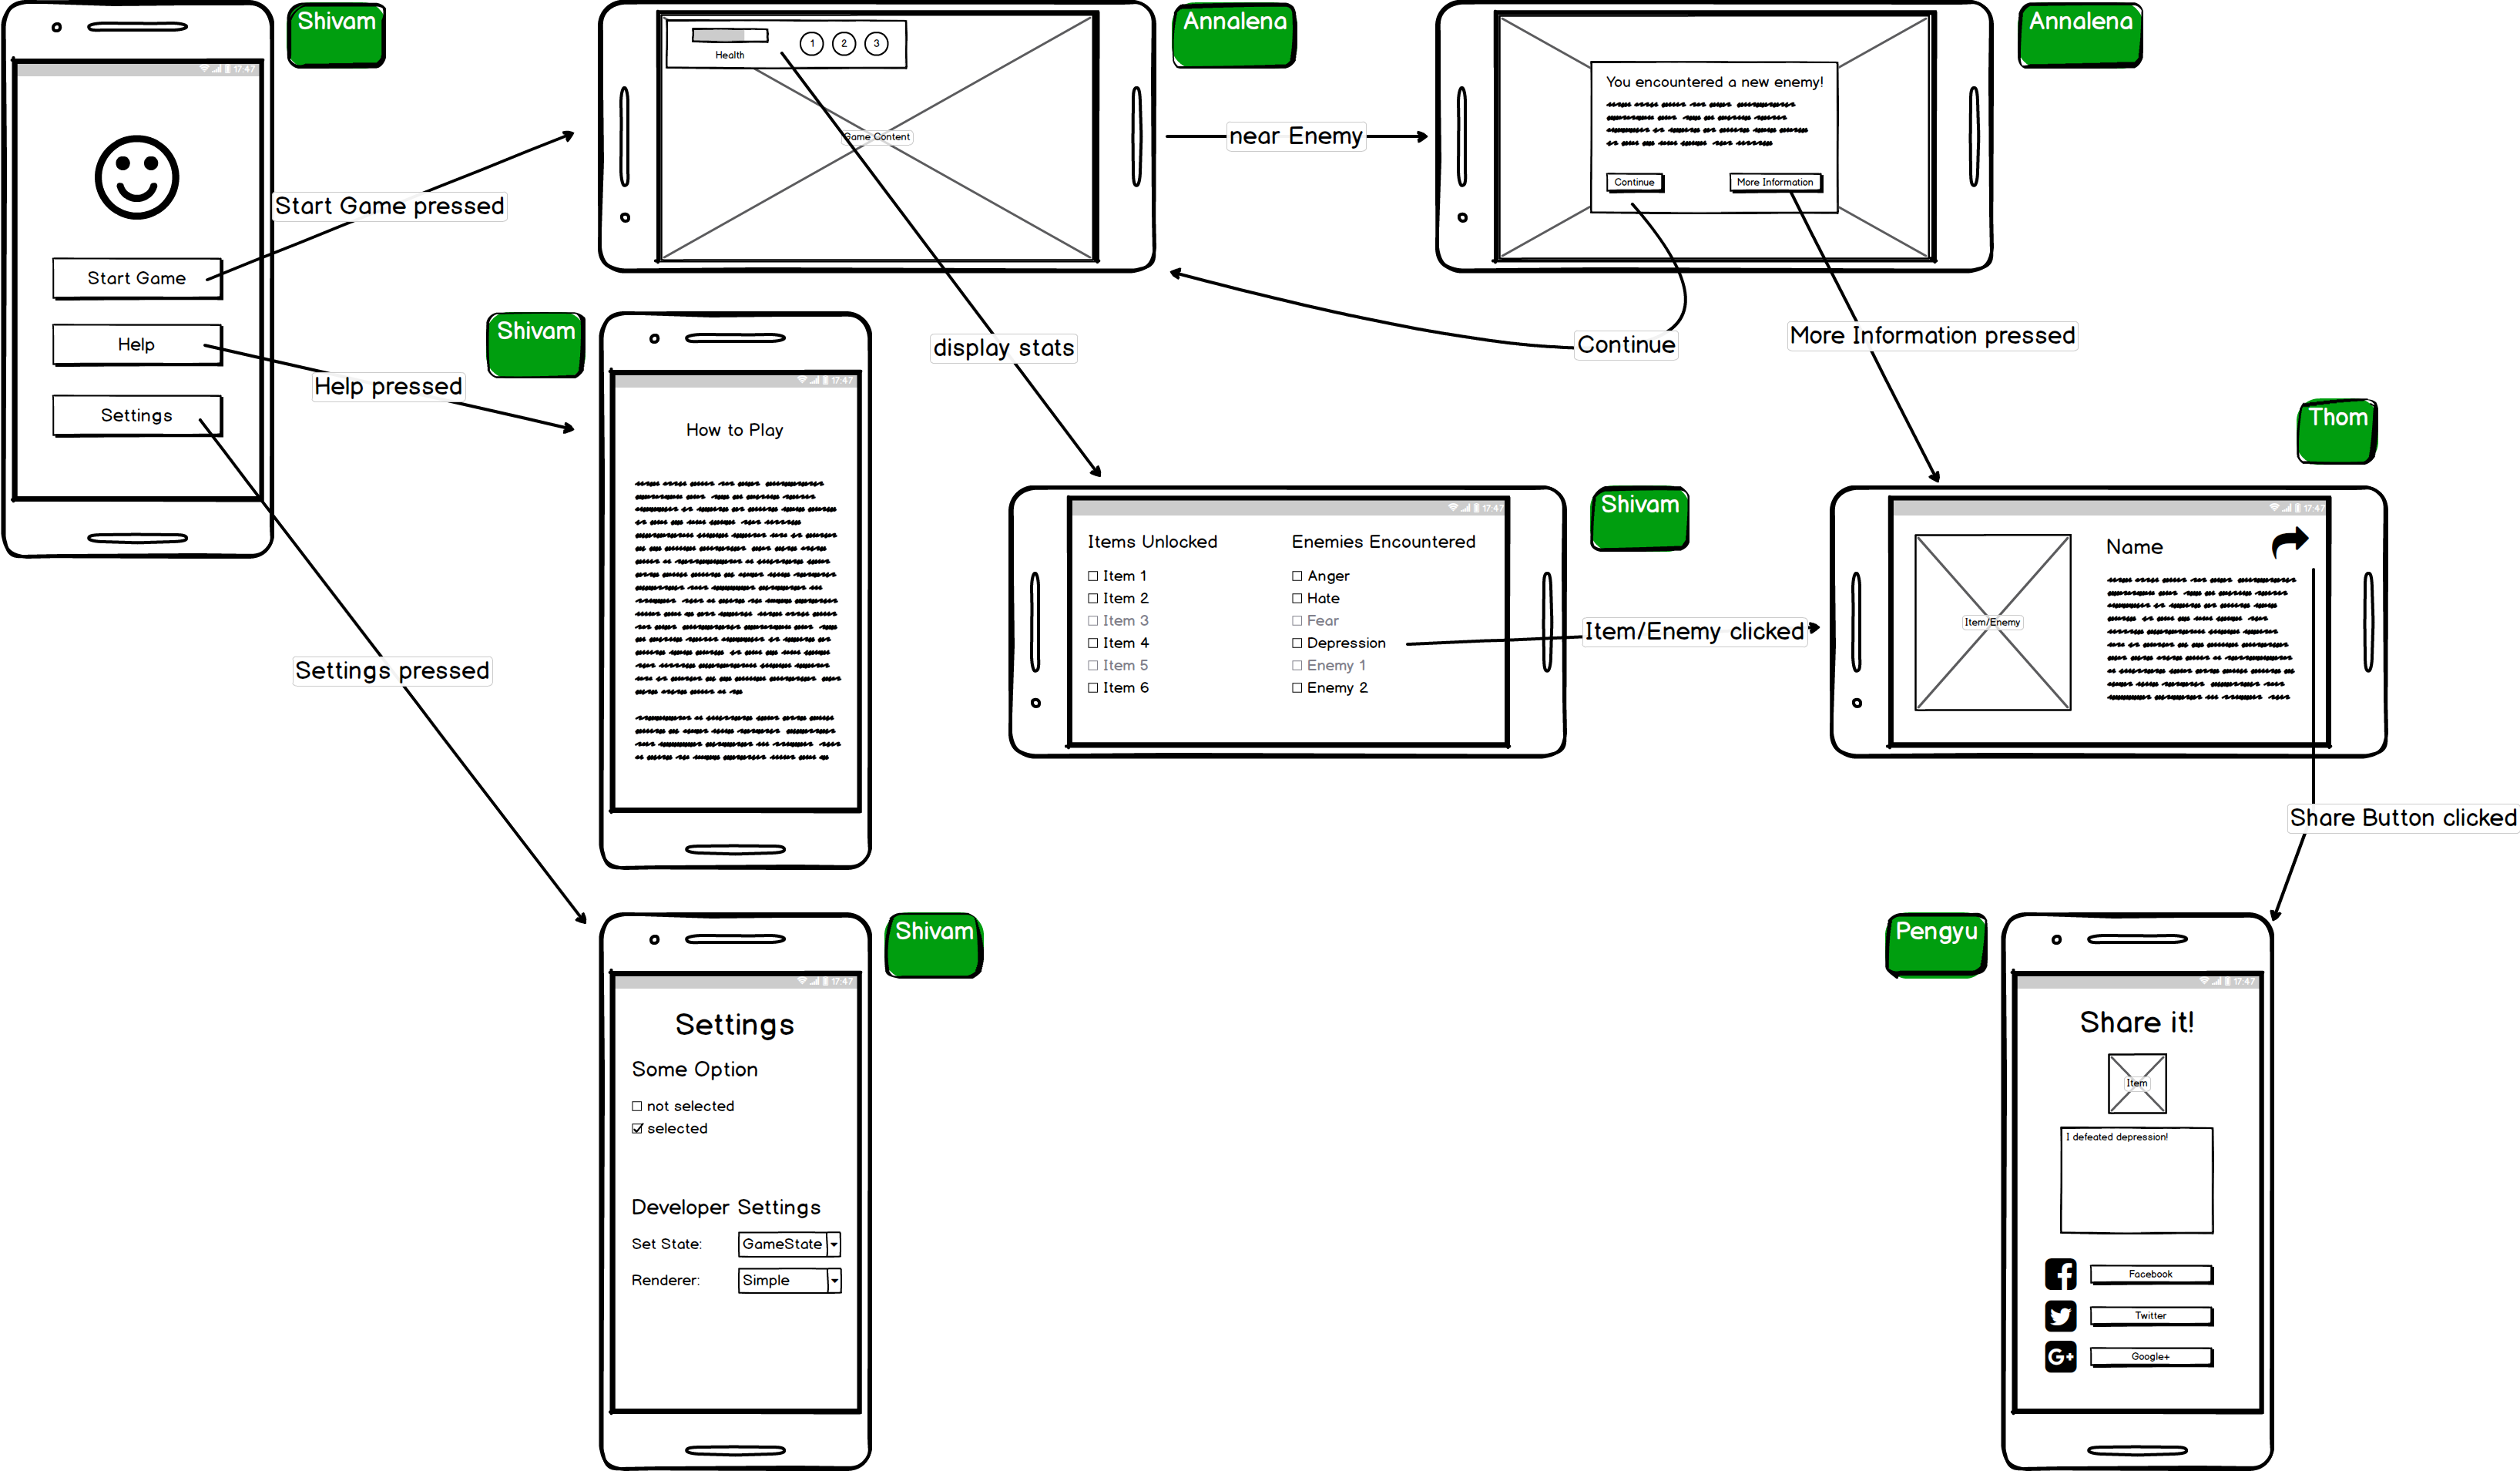
\includegraphics[width=7in]{figures/UIDesign/Storyboard.png}
	\caption{A storyboard of the app created with Balsamiq Mockups}
\end{figure*}
The application consists of seven different views in total. An overwiew of those views and the transitions between them is given in figure \ref{fig:storyboard}. At the beginning you see a \textbf{main menu} with the options to start the game, read the instructions on how to play and adapt some settings.

The \textbf{game view} contains the current level and some vital information for the gameplay like health and available attacks. The game dynamics are as follows: The state of the game changes based on the weather. In the current configuration it supports the three states sunny, rainy and snowy. The user can move the avatar by tilting the mobile device to the left or right. To jump the left side of the screen has to be touched and to attack the right side. The height of the jump can be controlled by the length of the touch, but is limited to a maximum jumptime.

The player has one standard attack, but can gain special attacks by defeating enemies. These special attacks come in three categories reflecting the three game states and give the player a certain bonus or malus depending on the type of enemy it is used against as shown in figure \ref{fig:attacks}. As these attacks are more usefull against enemies in a different state, the player is encouraged to wait for the weather status to change throughout the level.

\begin{figure}
\label{fig:attacks}
	\centering
	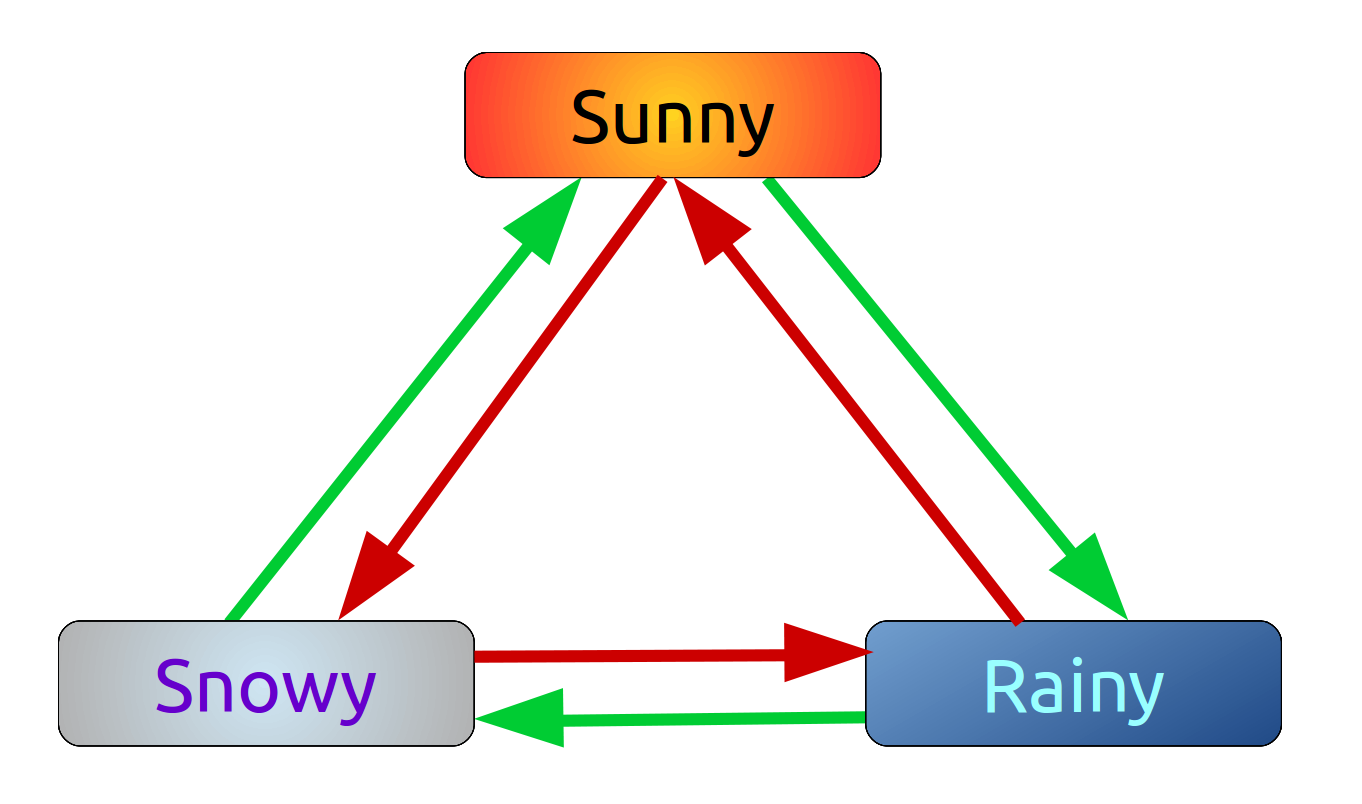
\includegraphics[width=0.9\columnwidth]{figures/attacks.png}
\end{figure}

During a level the player can also collect various pick-up items. Whenever a new item or enemy is encountered a message pops up giving the user the option to view more detailed information about this item or enemy. By clicking onto \textit{some symbol next to the players health bar} the user can review statistics like which items he/she already collected.

TODO: Stats view description

TODO: Info view description

TODO: Share view description

\section{Implementation}

This section will go more in detail on what we've built and how we've built it in regards to the Zen-Ze application. We won't cover the code in detail but we will focus on architecture and design.

For the full source code please refer to \url{https://github.com/Zen-Ze/ZenZe}.

\subsection{Key Features \& Technical Achievements}
Our application being a game, there are quite a few aspects we had to cover in terms of Game Design. For this ANNALENA SPEAK ABOUT IT HERE PLS (speak about sensors usage, the game engine you built...). 

Additionally, we decided to implement a database with our application. We wanted to have a simple and effective way of storing data from the application directly on the phone. For this we used the built-in SQLITE database that comes with Android. To implement this database in our application, we created a back-end package and added a library (the room persistence library \url{https://developer.android.com/topic/libraries/architecture/room.html}) to the project. The library in itself helped us create an interface between the Java application and the SQL. In this library, we define models (named entities), which are Java objects to which the data from the tables in the database will be transformed, but also Daos which are interfaces to create CRUD (create, read, update, delete) operations for our objects in the database. As for the database scheme, please find it enclosed at the end of the document.

Another key feature is the use of the OpenWeatherMap API. Our application relies on the weather and displays graphics based off it. For this we thus had to use some sort of service which would give us the weather and from this service inform the application. We used the OpenWeatherMap API for that as it's an API we had used in class and it seemed to fit our needs. One of the limitations with this API is though that we will not be able to publish the application to the play store, unless we pay OpenWeatherMap to be allowed to do more daily queries to the API. 

Finally, a key feature we added was the GPS. This was required for the weather service to be called properly as we queried the weather using the longitude and latitude of a location. For this we used the google play services library (\url{https://developer.android.com/training/location/index.html}) in order to retrieve a Location object of the last known location when the app is launched. 

\subsection{Key Lessons}
In this project, we have learned many things, in terms of coding for android, designing an application from scratch, understanding the concepts behind android... Out of all we learned, there are noticeable lessons we've gathered from this project. 

The first noticeable one was to comment our code properly so others could read and understand it, either with checking the files or by reading through the generated documentation. Additionally, we've learned to work as a team on different parts of the application, thus communication was key throughout the project.
Another part in which we learned a lot was with the overall design thinking process with each members finding 10 different ideas and gathering them to find the best one of them all.

\section{Project closeout}

%\begin{figure}
%\label{fig:figure1}
%\centering
%  
\includegraphics[width=0.9\columnwidth]{figures/sigchi-logo}
%  \caption{caption}
%\end{figure}
%
%This is a citation~\cite{acm_categories,ethics,Klemmer:2002:WSC:503376.503378}.\\
%This is a reference~\ref{fig:figure1}.\\
%This is a link \url{http://chi2016.acm.org/accessibility}.\\
%This is a ``quotation''.\\
%
%\begin{quote}
%This is a longer quote.  
%\end{quote}
%
%\begin{table}
%  \centering
%  \begin{tabular}{l r r r}
%    % \toprule
%    & & \multicolumn{2}{c}{\small{\textbf{Test Conditions}}} \\
%    \cmidrule(r){3-4}
%    {\small\textit{Name}}
%    & {\small \textit{First}}
%      & {\small \textit{Second}}
%    & {\small \textit{Final}} \\
%    \midrule
%    Marsden & 223.0 & 44 & 432,321 \\
%    Nass & 22.2 & 16 & 234,333 \\
%    Borriello & 22.9 & 11 & 93,123 \\
%    Karat & 34.9 & 2200 & 103,322 \\
%    % \bottomrule
%  \end{tabular}
%  \caption{Table caption}~\label{tab:table1}
%\end{table}
%
%\begin{itemize}
%\item item 1
%\item item 2
%\end{itemize}
%
%\begin{enumerate}
%\item enum 1
%\item enum 2
%\end{enumerate}

\section{Conclusion}


\section{Acknowledgments}
Lorem ipsum dolor sit amet, consectetur adipiscing elit, sed do eiusmod tempor incididunt ut labore et dolore magna aliqua. Ut enim ad minim veniam, quis nostrud exercitation ullamco laboris nisi ut aliquip ex ea commodo consequat. Duis aute irure dolor in reprehenderit in voluptate velit esse cillum dolore eu fugiat nulla pariatur. Excepteur sint occaecat cupidatat non proident, sunt in culpa qui officia deserunt mollit anim id est laborum.

% Balancing columns in a ref list is a bit of a pain because you
% either use a hack like flushend or balance, or manually insert
% a column break.  http://www.tex.ac.uk/cgi-bin/texfaq2html?label=balance
% multicols doesn't work because we're already in two-column mode,
% and flushend isn't awesome, so I choose balance.  See this
% for more info: http://cs.brown.edu/system/software/latex/doc/balance.pdf
%
% Note that in a perfect world balance wants to be in the first
% column of the last page.
%
% If balance doesn't work for you, you can remove that and
% hard-code a column break into the bbl file right before you
% submit:
%
% http://stackoverflow.com/questions/2149854/how-to-manually-equalize-columns-
% in-an-ieee-paper-if-using-bibtex
%
% Or, just remove \balance and give up on balancing the last page.
%
\balance{}

\bibliographystyle{SIGCHI-Reference-Format}
\bibliography{references}

\end{document}
